\documentclass[aspectratio=169,11pt]{beamer}
\usepackage[T1]{fontenc}
\usepackage{lmodern,booktabs,listings,amsmath,tikz}
\usetikzlibrary{arrows.meta,positioning}
\definecolor{ink}{HTML}{17324D}
\definecolor{accent}{HTML}{007F86}
\setbeamercolor{structure}{fg=accent}
\setbeamercolor{frametitle}{fg=ink}
\setbeamercolor{normal text}{fg=ink,bg=white}
\setbeamertemplate{navigation symbols}{}
\setbeamertemplate{footline}{\hfill\insertframenumber\hspace{5mm}\vspace{3mm}}
\setbeamertemplate{itemize items}[circle]
\setbeamersize{text margin left=8mm,text margin right=8mm}
\lstset{basicstyle=\ttfamily\small,breaklines=true,columns=fullflexible,keepspaces=true,showstringspaces=false}
\tikzset{stage/.style={draw=accent,rounded corners=2pt,minimum height=9mm,align=center,inner sep=5pt}, flow/.style={-{Stealth[length=2mm]},thick,draw=accent}}
\title{YOLOv4 in Remora: GPU backend experiments}
\author{MOCHA}
\date{September 2026}
\begin{document}

\begin{frame}{Executive summary}
\begin{center}
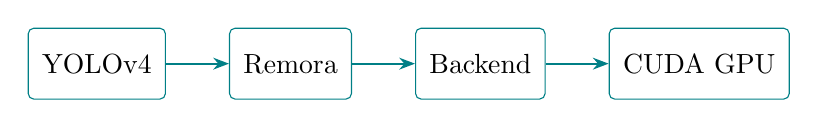
\begin{tikzpicture}[node distance=8mm]
\node[stage] (y) {YOLOv4};
\node[stage,right=of y] (r) {Remora};
\node[stage,right=of r] (b) {Backend};
\node[stage,right=of b] (g) {CUDA GPU};
\draw[flow] (y)--(r); \draw[flow] (r)--(b); \draw[flow] (b)--(g);
\end{tikzpicture}
\end{center}
\vspace{6mm}
\begin{itemize}\setlength\itemsep{6mm}
\item Experiment with different compilation targets for Remora.
\item Remora with PyTorch ran \textbf{5.4\% faster} than native Darknet in our comparison.
\end{itemize}
\note{45 seconds. We use YOLOv4 to compare compilation targets for Remora. The 5.4 percent figure is the latency reduction from 9.364 to 8.862 ms in the final report. It applies to our measured H200 configurations, not every possible Darknet configuration. All slide timings are the report's transfer-inclusive numbers, per image.}
\end{frame}

\begin{frame}{Experiment 1: original pipeline}
\begin{center}
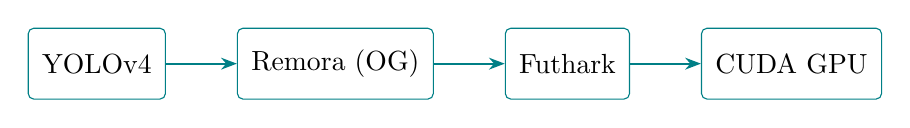
\begin{tikzpicture}[node distance=9mm]
\node[stage] (y) {YOLOv4};
\node[stage,right=of y] (r) {Remora (OG)};
\node[stage,right=of r] (f) {Futhark};
\node[stage,right=of f] (g) {CUDA GPU};
\draw[flow] (y)--(r); \draw[flow] (r)--(f); \draw[flow] (f)--(g);
\end{tikzpicture}
\end{center}
\vspace{5mm}
\begin{itemize}\setlength\itemsep{5mm}
\item Start with YOLOv4 written in Remora. \textbf{OG} denotes the original source.
\item Compile through Futhark to CUDA and run on one H200 GPU.
\item Compare against native Darknet C++.
\end{itemize}
\vfill
{\scriptsize Remora source: \texttt{examples/darknet/yolov4.remora}\\
Commit \texttt{72510c69006b90d1d5bcd1c472a69212b89b3116}, August 17, 2026.}
\note{65 seconds. Explain the common setup orally: one H200, 608 by 608 image, batch one, official weights, FP32. Image upload and decoded-output download are included, weights retained. Full network plus dense decoding, without NMS, loading, compilation or warmup. Three rounds of 30 calls following five warmups, median of round medians. cuDNN is off for Darknet and PyTorch, TF32 off. Source and timings: final report supplied September 16.}
\end{frame}

\begin{frame}{Original pipeline: results}
\begin{center}
\renewcommand{\arraystretch}{1.35}
\begin{tabular}{@{}lr@{}}
\toprule
Pipeline & Time (ms)\\\midrule
Remora (OG) $\rightarrow$ Futhark & 911.595\\
Darknet C++ & 9.364\\\bottomrule
\end{tabular}
\end{center}
\vspace{6mm}
\begin{itemize}
\item Original Remora through Futhark is about $100\times$ slower.
\end{itemize}
\vspace{8mm}
{\large\color{accent}Can we improve the Remora code?}
\note{55 seconds. Both rows include dense box decoding, with the same timing boundaries. These are our report measurements, not the later reproduction of Draper's original Darknet harness, which has different boundaries. The exact ratio is about 97.4, rounded to 100 for presentation.}
\end{frame}

\begin{frame}{Experiment 2: optimized Remora}
\begin{center}
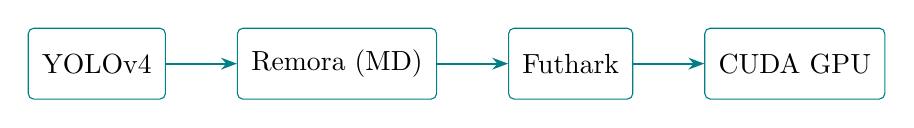
\begin{tikzpicture}[node distance=9mm]
\node[stage] (y) {YOLOv4};
\node[stage,right=of y] (r) {Remora (MD)};
\node[stage,right=of r] (f) {Futhark};
\node[stage,right=of f] (g) {CUDA GPU};
\draw[flow] (y)--(r); \draw[flow] (r)--(f); \draw[flow] (f)--(g);
\end{tikzpicture}
\end{center}
\vspace{5mm}
\begin{itemize}\setlength\itemsep{5mm}
\item \textbf{MD} is our modified Remora source in \texttt{remora-copy}.
\item Replace \texttt{reduce} with \texttt{reduce/zero} in dot products, giving the sum an explicit starting value of zero.
\item This exposes the reduction in a form the compiler can optimize more effectively.
\end{itemize}
\note{80 seconds. This is our measured modified source, not the teammate variant. Explain that dot products multiply corresponding elements and sum those products. reduce/zero supplies the additive identity explicitly. The source also contains a pooling rewrite, omitted from the slide as requested. Do not claim the table isolates the reduction change alone: these are the full modified-source measurements from the report. The teammate's additional nested pool reductions did not materially change whole-network timing.}
\end{frame}

\begin{frame}{Optimized Remora: results}
\begin{center}
\renewcommand{\arraystretch}{1.35}
\begin{tabular}{@{}lr@{}}
\toprule
Pipeline & Time (ms)\\\midrule
Remora (OG) $\rightarrow$ Futhark & 911.595\\
Remora (MD) $\rightarrow$ Futhark & 482.714\\
Darknet C++ & 9.364\\\bottomrule
\end{tabular}
\end{center}
\vspace{5mm}
\begin{itemize}\setlength\itemsep{3mm}
\item About $1.9\times$ faster than the original Remora pipeline.
\item Still about $52\times$ slower than Darknet.
\end{itemize}
\vspace{5mm}
{\large\color{accent}What if we try a different backend?}
\note{55 seconds. The modified source cuts latency by about 47 percent, or 1.89 times speedup. Its remaining gap motivates testing existing high-level GPU backends. Preserve these report numbers; the later Futhark version and teammate tests are separate experiments.}
\end{frame}

\begin{frame}{Experiment 3: alternative backends}
\begin{center}
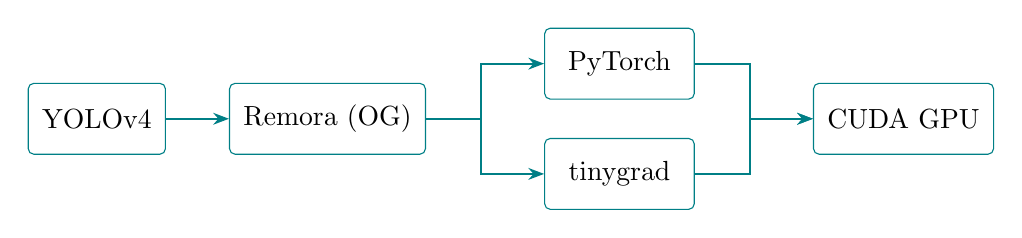
\begin{tikzpicture}[node distance=8mm]
\node[stage] (y) {YOLOv4};
\node[stage,right=of y] (r) {Remora (OG)};
\node[stage,minimum width=19mm,anchor=west] (p) at ([xshift=15mm,yshift=7mm]r.east) {PyTorch};
\node[stage,minimum width=19mm,anchor=west] (t) at ([xshift=15mm,yshift=-7mm]r.east) {tinygrad};
\node[stage,anchor=west] (g) at ([xshift=15mm,yshift=-7mm]p.east) {CUDA GPU};
\draw[flow] (y)--(r);
\draw[flow] (r.east) -- ++(7mm,0) |- (p.west);
\draw[flow] (r.east) -- ++(7mm,0) |- (t.west);
\draw[flow] (p.east) -- ++(7mm,0) |- (g.west);
\draw[flow] (t.east) -- ++(7mm,0) |- (g.west);
\end{tikzpicture}
\end{center}
\vspace{3mm}
\begin{itemize}\setlength\itemsep{4mm}
\item Built a small, specialized compiler for Remora YOLOv4 as a \textbf{rapid prototype}.
\item Read the Remora AST and map supported definitions to high-level PyTorch or tinygrad operations.
\item Establish an \textbf{end-to-end} comparison using existing backend operations, without advanced compiler techniques or SIMD/MIMD analysis.
\end{itemize}
\note{95 seconds. Python is omitted from the diagram for simplicity; the compiler still emits Python that calls the backend runtime. Recognition uses known function names with pinned AST fingerprints, not general semantic discovery. Composite calls and shapes are resolved from the source. High-level backend operations are important to performance. The prototype does not perform its own SIMD/MIMD analysis, though the backend implementations have their own optimizations. Correctness was tested on seven inputs: all passed the original dense check; on the six additions all pipelines retained the same candidate IDs and classes after common filtering and NMS, despite numerical differences. Do not describe the compiler as proven correct for arbitrary Remora programs.}
\end{frame}

\begin{frame}{Alternative backends: results}
\begin{center}
\renewcommand{\arraystretch}{1.05}
\begin{tabular}{@{}lr@{}}
\toprule
Pipeline & Time (ms)\\\midrule
Remora (OG) $\rightarrow$ PyTorch & 8.862\\
Direct PyTorch & 8.927\\
Remora (OG) $\rightarrow$ tinygrad & 156.294\\
Direct tinygrad & 156.301\\
Darknet C++ & 9.364\\\bottomrule
\end{tabular}
\end{center}
\vspace{1mm}
\begin{itemize}\setlength\itemsep{2mm}
\item Remora with PyTorch is \textbf{5.4\% faster} than Darknet. Both backends closely match their direct implementations.
\item Rapid prototyping gives us an end-to-end baseline for future Futhark/MLIR compilation and scheduling work.
\item We checked all pipelines for correctness. After NMS, all kept the same candidate boxes and classes on the tested inputs.
\end{itemize}
\note{95 seconds. The PyTorch advantage is specific to our measured configuration; tinygrad is substantially slower. Generated versus direct differences are small and should not be interpreted as Remora intrinsically accelerating the backend. Direct implementations construct the network independently from Darknet's configuration but share the runtime operations. Optimized tinygrad rows remain omitted as requested earlier. End-to-end here means the source-to-GPU compilation path and measured network-plus-decoding execution, not whole-program startup or a service including NMS. These results establish an achievable baseline rather than a theoretical performance upper bound.}
\end{frame}

\begin{frame}{Next semester}
\begin{itemize}\setlength\itemsep{5mm}
\item Explore \textbf{AI-enabled compilation}: use AI to investigate which compiler technologies suit a language and its workloads.
\item Use AI to help build compilers, extending our Remora backend prototype.
\item Use AI as a separate pass to generate or improve compiled code for specific programs, building on experiments such as \texttt{reduce/zero}.
\item Explore a general framework for these approaches with MLIR and other compilation targets.
\end{itemize}
\note{110 seconds. Distinguish AI as a tool for developing the compiler from AI as a separate pass that proposes program-specific transformations. The reduce/zero experiment is an example of the kind of source rewrite to explore, not evidence of an already implemented automatic AI pass. A future framework should evaluate proposed transformations for correctness and performance. The broader goal is to learn which compiler technology is useful for a particular source language and workload, then apply the process beyond YOLOv4 and beyond the current backends.}
\end{frame}
\end{document}
